%%---------------------------------------------------------------------
%	Preamble
%	AMS gruppe 12
%	AMS F18
%---------------------------------------------------------------------
\documentclass[12pt,fleqn,a4paper]{article}
\usepackage[utf8]{inputenc}
\usepackage[danish]{babel}
\usepackage[top=2.5cm, left=2cm, right=2cm, bottom=2.5cm]{geometry}
\usepackage{graphicx}
\usepackage[bottom]{footmisc}
\usepackage{framed}
\usepackage{caption}
\usepackage{float}
\usepackage{mdframed}
\usepackage{listings}
\usepackage{color}
\usepackage[T1]{fontenc}
\usepackage{amsmath,amsfonts,amsthm} % Math packages
\usepackage{array}
\usepackage{wrapfig}
\usepackage{multirow}
\usepackage{tabu}
\usepackage{longtable}
\usepackage{lastpage}
\usepackage{fancyhdr}
\usepackage[compact]{titlesec}
\usepackage[table,xcdraw]{xcolor}
\usepackage{arydshln}
\usepackage[isbn,issn,url]{dk-bib}
\usepackage[toc,page]{appendix}
\usepackage{url}
\def\UrlBreaks{\do\/\do-}

\definecolor{mygreen}{RGB}{28,172,0} % color values Red, Green, Blue
\definecolor{mylilas}{RGB}{170,55,241}
\renewcommand{\lstlistingname}{Kodeudsnit}
\tabulinesep=3mm

\setcounter{secnumdepth}{2}
\setcounter{tocdepth}{2}

\setlength{\parindent}{0mm} %intet indryk
\setlength{\parskip}{3mm} 	%linjeskift v. afsnit

% Ændring af enumerize og itemize 
\usepackage{enumitem} % @http://ctan.org/pkg/enumitem
\setlist[itemize]{topsep=0pt, itemsep=0.5pt}
\setlist[enumerate]{topsep=0pt, itemsep=0.5pt}

%afstand omkring sections
\titlespacing{\section}{0pt}{5mm}{0pt}
\titlespacing{\subsection}{0pt}{2mm}{0pt}
\titlespacing{\subsubsection}{0pt}{2mm}{0pt}

\usepackage{arydshln}
%aryd
\setlength\dashlinedash{3pt}
\setlength\dashlinegap{4pt}

\lstset{language=C++,
	breaklines=true,
	keywordstyle=\color{blue},
	stringstyle=\color{red},
	commentstyle=\color{mygreen},
	morecomment=[l][\color{magenta}]{\#}
}

%header & footer
\makeatletter
\pagestyle{fancy}
\fancypagestyle{plain}{}
\renewcommand{\chaptermark}[1]{\markboth{#1}{}}
\setlength{\headheight}{35pt}
\fancyfoot{} % clear all fields
\fancyfoot[R]{Side \thepage\ af \pageref{LastPage}}
\fancyhead{} % clear all fields
\fancyhead[L]{
\includegraphics[clip, trim = 0 0 240pt 0, height=30pt]{Figur/IHA_AU_logo.png}}
\fancyhead[R]{Forår 2018}
\fancyhead[C]{Anvendte Microcontroller Systemer}
\renewcommand{\headrulewidth}{0pt}

\def\thickhrulefill{\leavevmode \leaders \hrule height 1.2ex \hfill \kern \z@}
\def\@makechapterhead#1{
  \vspace*{10\p@}%
  {\parindent \z@ \centering \reset@font
        \thickhrulefill\quad 
        \scshape\bfseries\textit{\@chapapp{}  \thechapter}  
        \quad \thickhrulefill
        \par\nobreak
        \vspace*{10\p@}%
        \interlinepenalty\@M
        \hrule
        \vspace*{10\p@}%
        \Huge \bfseries #1 \par\nobreak
        \par
        \vspace*{10\p@}%
        \hrule
        \vskip 40\p@
  }}

\usepackage{tcolorbox}
\definecolor{mycolor}{rgb}{0.122, 0.435, 0.698}% Rule colour
\makeatletter
\newcommand{\mybox}[1]{%
	\setbox0=\hbox{#1}%
	\setlength{\@tempdima}{\dimexpr\wd0+13pt}%
	\begin{tcolorbox}[colframe=mycolor,boxrule=0.5pt,arc=4pt,
		left=6pt,right=6pt,top=6pt,bottom=6pt,boxsep=0pt]
		#1
	\end{tcolorbox}
}
\makeatother

\graphicspath{ {Figur/} }


%Se Kodeudsnit \ref{lstlisting:generel_kode}

%\captionof{lstlisting}{Generelle egenskaber for koden til fremstilling af diverse figure i matlab} 
%\label{lstlisting:generel_kode}
%\vspace{5mm} %5mm vertical space
%
%\subsection{Kode til lyd i forhold til tiden}
%\begin{framed}
%\begin{center}
%\begin{lstlisting}
%figure('name','trafikstoejen i fuld laengde'); clf
%subplot(211);
%plot(t,s_sound_left)
%xlabel('Tid (sek)')
%ylabel('Signalstyrke')
%title('Trafikstoej set i forhold til tiden')
%grid on
%hold on
%\end{lstlisting}
%\end{center}
%\end{framed}




%\begin{document}

\chapter{Enhedstests og Integrationstest af PSoC}
\label{appendix:BilagPSoCEnhedstests}

I dette dokument kan de forskellige enhedstest, der er lavet til PSoC'en beskrevet.

\section{Enhedstest af Motorkontrol}
For at teste motorkontrollen, så analyseres signalerne fra motorkontrollen med et oscilloskop.
\\Der måles på signalerne når motorerne er sat til at køre fremad og dreje venstre om.
\\Testen er gennemført, hvis motorerne opfylder følgende:

\begin{table}[H]
\centering
\begin{tabular}{|l|c|c|c|}
\hline
Køreretning & LeftForward & LeftBackward & EnableLeft                                   \\ \hline
Fremad      & Høj         & Lav          & PWM signal                                   \\ \hdashline
Venstre om  & Lav         & Høj          & PWM signal, duty cycle lavere end ved fremad \\ \hline
\end{tabular}
\caption{Krav til enhedstest af motorkontrol}
\label{motorkontrolenhedstest}
\end{table}

Resultaterne af testen ses på figur \ref{fig:enhedstest_motorstyring}.

\begin{figure}[H] %billede af tests
\centering
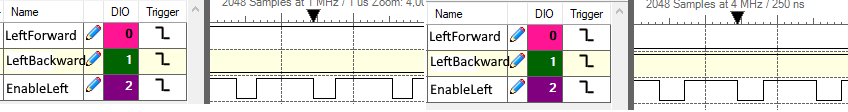
\includegraphics[width = 0.8\textwidth]{MotorstyringTest.png}
\caption{Test af motorstyringen med oscilloskop, ved hhv. fremad og venstre om}
\label{fig:enhedstest_motorstyring}
\end{figure}

Ud fra ovenstående figur kan det konkluderes, at motorkontrollen gør som ønsket.

\section{Enhedstest af regulering}
For at teste af reguleringen virker som ønsket laves der en test, hvor der med oscilloscop måles på tandhjulenes frekvens med og uden regulering. Testen laves efter hjulene har kørt fremad i 10 sekunder, for at garantere, at hastigheden er stabil.
\\Testen er bestået, hvis reguleringen markant reducerer forskellen mellem frekvenserne.
Resultatet af testen ses på figur \ref{fig:test_motor_uden} og \ref{fig:test_motor_med}.
\begin{figure}[H]  %BILLEDE AF TEST!!!
\centering
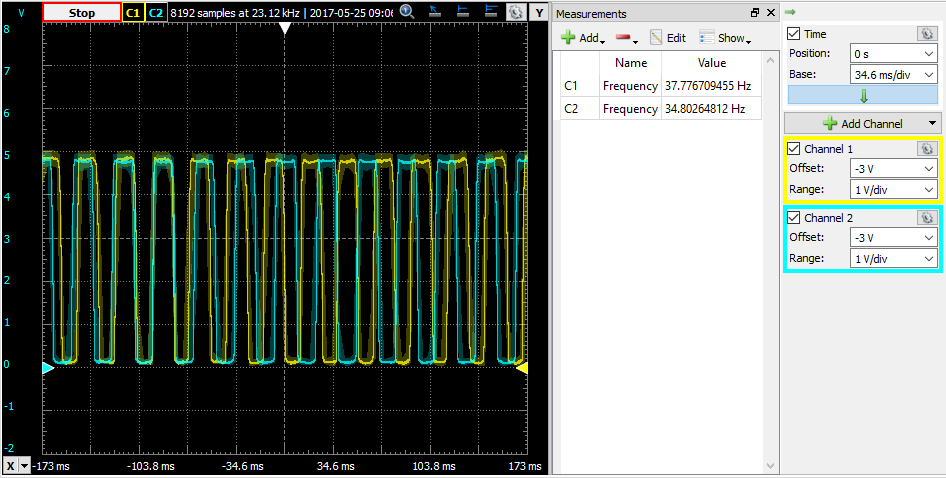
\includegraphics[clip, trim = 0cm 0cm 0cm 0cm , width = \textwidth]{test_motor_uden.png}
\caption{Test af motorer, uden regulering}
\label{fig:test_motor_uden}
\end{figure}
Ovenstående figur viser frekvensen, hvorved lyset kommer igennem tandhjulets takker. Det kan ses, at der næsten er en frekvensforskel på 3 Hz imellem hjulene. Ud fra hastighedsformlen i rapporten kan det udregnes, at dette vil lave en forskel på 4cm mellem hjulenes tilbagelagte distance i sekundet.
\begin{figure}[H]  %BILLEDE AF TEST!!!
\centering
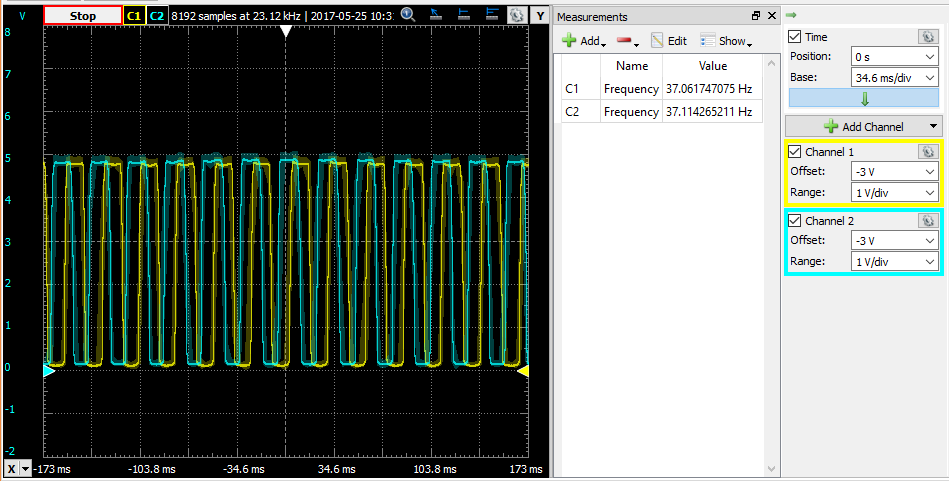
\includegraphics[clip, trim = 0cm 0cm 0cm 0cm , width = \textwidth]{test_motor_med.png}
\caption{Test af motorer, med regulering}
\label{fig:test_motor_med}
\end{figure}

Ovenstående figur viser, at efter reguleringen er sat ind, så er forskellen mellem hjulenes frekvens nærmest helt forsvundet. Det kan altså konkluderes, at reguleringen virker som ønsket.

\section{Integrationstest af I2C mellem PSoC og Raspberry pi}
For at teste I2C forbindelsen laves en test, hvor der sendes beskeder mellem PSoC og kontrolenhed.
Testen er gennemført, hvis det er muligt at sende og modtage beskeder mellem de to enheder.

Resultatet af testen kan ses på \ref{fig:test_i2c_read} og \ref{fig:test_i2c_write}.

\begin{figure}[H]  %BILLEDE AF TEST!!!
\centering
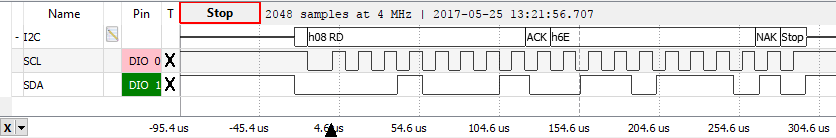
\includegraphics[width=\textwidth]{test_i2c_read.png}
\caption{En read-besked sendt over I2C-linjen}
\label{fig:test_i2c_read}
\end{figure}

På figur \ref{fig:test_i2c_read} ses en gennemført read transaktion, hvor kontrolenheden først sender adresse og fortæller, at den ønsker at læse. PSoC'en svarer med et acknowledge, hvorefter den sender indholdet af dens read-buffer. 

\begin{figure}[H]  %BILLEDE AF TEST!!!
\centering
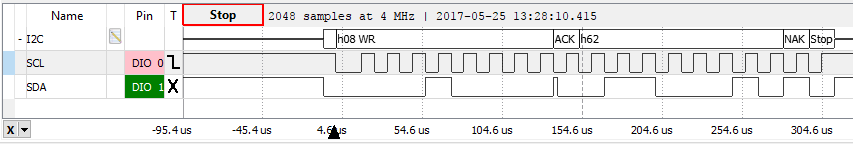
\includegraphics[width = \textwidth]{test_i2c_write.png}
\caption{En write-besked sendt over I2C-linjen}
\label{fig:test_i2c_write}
\end{figure}

På figur \ref{fig:test_i2c_write} ses en gennemført write transaktion.

Da begge beskeder bliver sendt succesfuldt, kan det konkluderes, at kommunikationslinjen virker som ønsket.

%\end{document}